% SPDX-License-Identifier: CC-BY-SA-4.0
% Author: Matthieu Perrin
% Part: 
% Section: 
% Sub-section: 
% Frame: 

\begingroup

\begin{frame}[fragile]{Consensus number de Common2}
  \vspace{-2mm}
  \begin{block}{Lemme}
    Tout objet de Common2 a un consensus number au plus égal à 2.
  \end{block}
  \begin{block}{Démonstration}
    Supposons qu'il existe un protocole pour 3 threads : $T_0$, $T_1$, $T_2$.
    \begin{itemize}
    \item Si l'un d'eux lit, écrit ou accède à un registre différent : comme avant
    \end{itemize}
    \begin{minipage}{.45\textwidth}
      \begin{itemize}
      \item Si $T_0$ et $T_1$ commutent
      \end{itemize}
      \begin{center}
        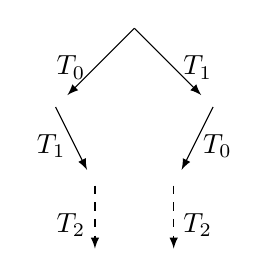
\begin{tikzpicture}
          
          \draw[-latex] (1.5,3) -- (0.65,2.15);
          \draw (1,2.5) node[left]{$T_0$};
          \draw[-latex] (1.5,3) -- (2.35,2.15);
          \draw (2,2.5) node[right]{$T_1$};
          
          \draw[-latex] (0.5,2) -- (0.9,1.2);
          \draw (0.75,1.5) node[left]{$T_1$};
          \draw[-latex] (2.5,2) -- (2.1,1.2);
          \draw (2.25,1.5) node[right]{$T_0$};
          
          \draw[-latex, dashed] (1,1) -- (1,0.2);
          \draw (1,0.5) node[left]{$T_2$};
          \draw[-latex, dashed] (2,1) -- (2,0.2);
          \draw (2,0.5) node[right]{$T_2$};
          
          %        \cstate{1.5,3}{red}{blue}
          % 
          %        \ustate{0.5,2}{red}
          %        \ustate{2.5,2}{blue}
          % 
          %        \ustate{1,1}{red}
          %        \ustate{2,1}{blue}
          % 
          %        \ustate{1,0}{red}
          %        \ustate{2,0}{blue}
          
        \end{tikzpicture}
      \end{center}
    \end{minipage}
    \begin{minipage}{.5\textwidth}
      \begin{itemize}
      \item Si $T_0$ écrase $T_1$
      \end{itemize}
      \begin{center}
        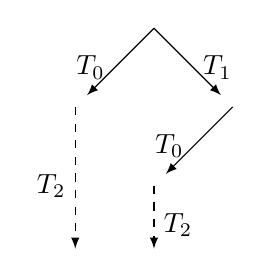
\begin{tikzpicture}
          
          \draw[-latex] (1,3) -- (0.15,2.15);
          \draw (0.5,2.5) node[left]{$T_0$};
          \draw[-latex] (1,3) -- (1.85,2.15);
          \draw (1.5,2.5) node[right]{$T_1$};
          
          \draw[-latex, dashed] (0,2) -- (0,0.2);
          \draw (0,1) node[left]{$T_2$};
          \draw[-latex] (2,2) -- (1.15,1.15);
          \draw (1.5,1.5) node[left]{$T_0$};
          
          \draw[-latex, dashed] (1,1) -- (1,0.2);
          \draw (1,0.5) node[right]{$T_2$};
          
          %    \cstate{1,3}{red}{blue}
          % 
          %    \ustate{0,2}{red}
          %    \ustate{2,2}{blue}
          % 
          %    \ustate{1,1}{blue}
          % 
          %    \ustate{0,0}{red}
          %    \ustate{1,0}{blue}
          
        \end{tikzpicture}
      \end{center}
    \end{minipage}
  \end{block}
\end{frame}

\endgroup
\endinput

